\documentclass[border=4pt]{standalone}

\usepackage{tikz}
\usepackage{pgfplots}
\usepackage{eso-pic}

\pgfplotsset{compat=1.18}

\usetikzlibrary{positioning,shapes.geometric,arrows,calc,math,angles,quotes,trees}

\tikzstyle{startstop} = [rectangle, rounded corners, minimum width=3cm, minimum height=1cm,text centered, draw=black, fill=red!30]

\tikzstyle{inputoutput} = [trapezium, trapezium left angle=70, trapezium right angle=110, minimum width=3cm, minimum height=1cm, text centered, draw=black, fill=blue!30]

\tikzstyle{quantum-process} = [rectangle, minimum width=3cm, minimum height=1cm, text centered, draw=black, fill=magenta!30]

\tikzstyle{classical-process} = [rectangle, minimum width=3cm, minimum height=1cm, text centered, draw=black, fill=orange!30]

\tikzstyle{decision} = [diamond, minimum width=3cm, minimum height=1cm, text centered, draw=black, fill=green!30]

\tikzstyle{decision2} = [diamond, minimum width=3cm, minimum height=1cm, text centered, draw=black, fill=green!30]

\tikzstyle{arrow} = [thick,->,>=stealth,line width=2.5pt]

\tikzstyle{qkds-level-1} = [rectangle, draw, fill=red!30, rounded corners, minimum height=3em]

\tikzstyle{qkds-level-2} = [rectangle, draw, fill=blue!30, rounded corners, minimum height=3em]

\tikzstyle{qkds-level-3} = [rectangle, draw, fill=green!30, rounded corners, minimum height=3em]

\begin{document}
    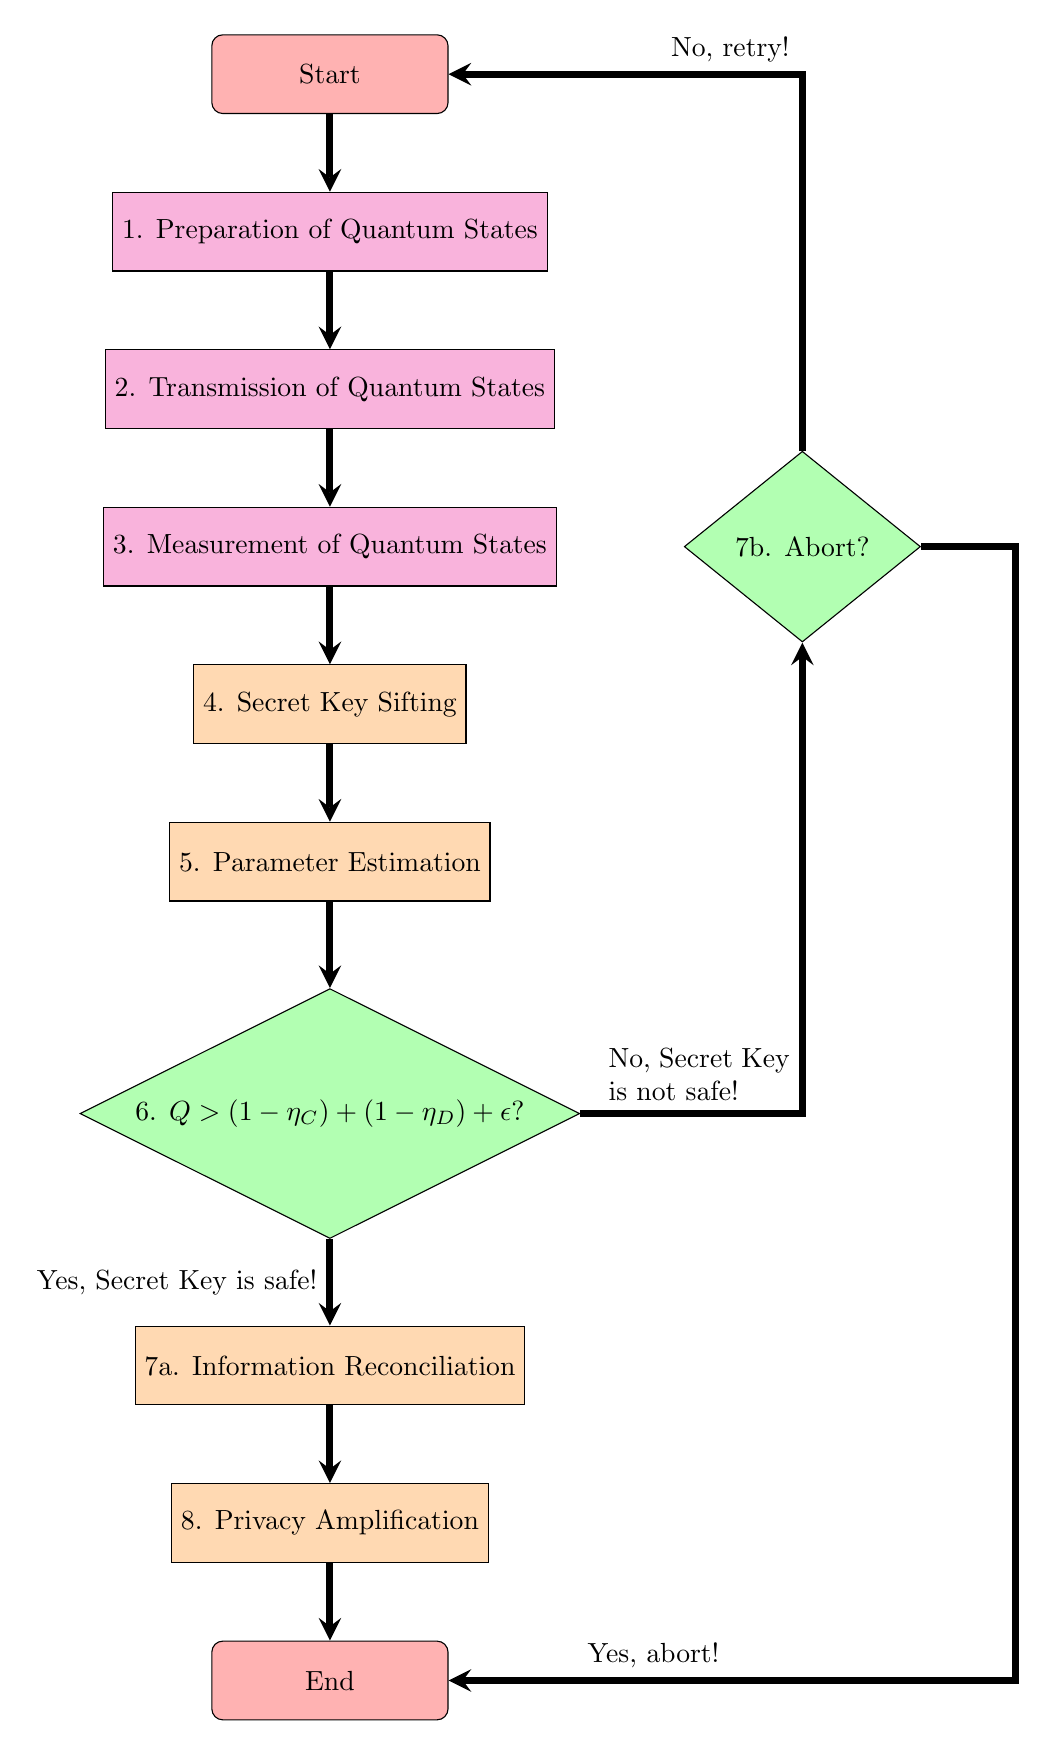
\begin{tikzpicture}[node distance=2cm]
        \node (start) [startstop] {Start};
        \node (preparation-of-quantum-states) [quantum-process,below of=start] { 1. Preparation of Quantum States };
        \node (transmission-of-quantum-states) [quantum-process,below of=preparation-of-quantum-states] { 2. Transmission of Quantum States};
        \node (measurement-of-quantum-states) [quantum-process,below of=transmission-of-quantum-states] { 3. Measurement of Quantum States };
        \node (secret-key-sifting) [classical-process,below of=measurement-of-quantum-states] { 4. Secret Key Sifting};
        \node (parameter-estimation) [classical-process,below of=secret-key-sifting] { 5. Parameter Estimation};
        \node (error-threshold-decision) [decision,below of=parameter-estimation, yshift=-1.2cm, aspect=2] { 6. $Q > (1 - {\eta}_{C}) + (1 - {\eta}_{D}) + \epsilon$?};
        \node (information-reconciliation) [classical-process,below of=error-threshold-decision, yshift=-1.2cm] { 7a. Information Reconciliation};
        \node (abort-decision) [decision2,right of=measurement-of-quantum-states, xshift=4cm] { 7b. Abort?};
        \node (privacy-amplification) [classical-process,below of=information-reconciliation] { 8. Privacy Amplification};
        \node (end) [startstop,below of=privacy-amplification] {End};
        
        \coordinate[right=of end, xshift=5.2cm] (aux-1);
        
        \draw [arrow] (start) -- (preparation-of-quantum-states);
        \draw [arrow] (preparation-of-quantum-states) -- (transmission-of-quantum-states);
        \draw [arrow] (transmission-of-quantum-states) -- (measurement-of-quantum-states);
        \draw [arrow] (measurement-of-quantum-states) -- (secret-key-sifting);
        \draw [arrow] (secret-key-sifting) -- (parameter-estimation);
        \draw [arrow] (parameter-estimation) -- (error-threshold-decision);
        \draw [arrow] (error-threshold-decision) -- node[anchor=east] {Yes, Secret Key is safe!}(information-reconciliation);
        \draw [arrow] (information-reconciliation) -- (privacy-amplification);
        \draw [arrow] (privacy-amplification) -- (end);
        \draw [arrow] (error-threshold-decision) -| node[anchor=south east] {\parbox{2.3cm}{No, Secret Key is not safe!}}(abort-decision);
        \draw [arrow] (abort-decision) -| (aux-1) -- node[anchor=south east] {Yes, abort!}(end);
        \draw [arrow] (abort-decision) |- node[anchor=south east] {No, retry!}(start);
    \end{tikzpicture}
\end{document}